% Dokumentklasse
% --------------
\documentclass[12pt,naustrian,a4widepaper]{scrartcl}   
% article style
%   - 11pt Schriftgroesse
%   - new austrian (neue Rechtschreibung)
%   - Papierformat A4
%   - pdf-hyperlinks

%****************In her all definitions are listed*********************
\usepackage[ngerman]{babel} 					% wegen deutschen Umlauten
\usepackage[utf8]{inputenc}
\usepackage{amsmath}
\usepackage[usenames,dvipsnames]{xcolor}
\usepackage{pdfpages}
\usepackage{lastpage} 							% Required to determine the last page for the footer
%\usepackage{amsmath}
\usepackage{float}
\usepackage{hyperref}
\usepackage{listings}
\usepackage{graphicx}							% Einbinden von Bildern
%\usepackage{multicol} 							% Spalten
%\usepackage{textcomp} 							% spitze klammern
%\usepackage{hyperref}  						% hyperlinks
\usepackage[absolute]{textpos}
\usepackage{xcolor}
\usepackage{tabularx}
\usepackage{tcolorbox}
\usepackage{enumitem}
\usepackage{fancyhdr}   % für Kopf- und Fusszeilen
%*************************************************************************
\pagestyle{fancy} 						% Wird für den Header gebraucht

% Seitenspiegel
% -------------

\typearea{8}	% Festlegung des Seitenspiegels gem. Koma. 4..groß, 9..klein


% Kopfzeile
% ---------
\lhead{{\footnotesize{\docauthor, \doccoauthor}}}   %  (links)
\chead{{\footnotesize{Systemdokumentation - \docproject}}} %  (mitte)
\rhead{{\footnotesize{Seite \thepage}}}      %  (rechts)

% Fusszeile
% ---------
\lfoot{}  % links
\cfoot{}  % mitte 
\rfoot{}  % rechts

% Absatzformatierung
% ------------------
\setlength{\parindent}{0cm}   % Einrückung der 1. Zeile jedes Absatzes
\setlength{\parskip}{10pt}    % Abstand zwischen den Absätzen

\selectlanguage{naustrian}   % oder "american" für engl. Texte

% Titelblatt
% ----------
\newcommand{\hgbtitle}{
\title {\vspace{1cm}
	
\includegraphics[width=8cm]{./Images/FhOOeLogoOkt2009_HSD_Rot_pastell}\\
	\vspace{2cm}
	{\textbf{Systemdokumentation\\Projekt \docproject}}\\
	\vspace{5mm}
	{\small{Version 1.0}}\\
	\vspace{5mm}
}

\author{\small{\docauthor, \doccoauthor}}
\date  {\small{Hagenberg, \today}}
\maketitle
}

%****************** self defined commands ***************************
%include a pseudocode file
%usage: \pseudocode{Title}{path_to_your_file/filename} (relative to Übung root folder)
\newcommand{\pseudocode}[2]{
\begin{itemize}
\item[]\lstinputlisting[caption="#1",label="#1", style=pseudocodeStyle]{../#2}
\end{itemize}
}

% Include Linux terminal output
% Usage: \linuxoutput{Title}{path_to_your_file/filename}
\newcommand{\linuxoutput}[2]{
	\begin{itemize}
		\item[]\lstinputlisting[
		caption="#1",
		label="#1",
		style=linuxStyle
		]{../#2}
	\end{itemize}
}

% include an ARM Assembly source file
% usage: \armasm{path_to_your_file/filename}
%        (relative to Übung root folder)
\newcommand{\armasm}[1]{
	\begin{itemize}
		\item[]\lstinputlisting[
		caption="#1.s",
		label="#1.s",
		style=armasm
		]{../#1.s}
	\end{itemize}
}

% Usage: \bashscript{Title}{path_to_script}
\newcommand{\bashscript}[2]{
	\begin{itemize}
		\item[]\lstinputlisting[caption="#1",label="#1",style=bashStyle]{../#2}
	\end{itemize}
}

%include a .cpp source file
%usage: \cpp{path_to_your_file/filename}(relative to Übung root folder)
\newcommand{\cpp}[1]{
\begin{itemize}
\item[]\lstinputlisting[caption="#1.cpp",label="#1.cpp", style=customcpp]{../#1.cpp}
\end{itemize}
}

%include a .c source file
%usage: \cfile{path_to_your_file/filename}(relative to Übung root folder)
\newcommand{\cfile}[1]{
	\begin{itemize}
		\item[]\lstinputlisting[caption="#1.c",label="#1.c", style=customcpp]{../#1.c}
	\end{itemize}
}

%include a .h source file
%usage: \h{path_to_your_file/filename} (relative to Übung root folder)
\newcommand{\h}[1]{
\begin{itemize}
\item[]\lstinputlisting[caption="#1.h",label="#1.h", style=customcpp]{../#1.h}
\end{itemize}
}

%include a module (.cpp and .h)
%usage: \cppmodule{path_to_your_file/filename} (relative to Übung root folder)
\newcommand{\cppmodule}[1]{
\begin{itemize}
\item[]\lstinputlisting[caption=#1.h,label=#1.h, style=customcpp]{../#1.h}
\item[]\lstinputlisting[caption=#1.cpp,label=#1.cpp, style=customcpp]{../#1.cpp}
\end{itemize}
}

%include a code snippet
%usage: \snippet{path_to_your_file/filename}{startline}{endline} (relative to Übung root folder)
\newcommand{\snippet}[3]{
\begin{itemize}
\item[]\lstinputlisting[caption=#1.cpp,label=#1.cpp, style=customcpp, firstline=#2,lastline=#3]{../#1.cpp}
\end{itemize}
}

%include a test-output file 
%usage: \testoutput{path_to_your_file/filename} (relative to Übung root folder)
\newcommand{\testoutput}[1]{
\begin{itemize}
\item[]\lstinputlisting[caption=#1]{../#1.txt}
\end{itemize}
}

%include a figure 
%usage: \fig{path_to_your_file/filename}{width}{caption text} (relative to Übung root folder)
%width between 0.0 - 1.0 -> correspond with textwidth
\newcommand{\fig}[3]{
\begin{figure}[H]
\centering
\includegraphics[width=#2\textwidth]{../#1}
\caption{#3}
\label{fig:fig1}
\end{figure}
}

%include a flowchart
%usage: \flow{path_to_your_file/filename} (relative to Übung root folder)
\newcommand{\flow}[3]{
\begin{figure}[H]
\centering
\includegraphics[width=0.5\textwidth]{../#1.png}
\caption{Flussdiagramm #1}
\label{fig:fig1}
\end{figure}
}


\lstset{
   literate      = 
      {á}{{\'a}}1  {é}{{\'e}}1  {í}{{\'i}}1 {ó}{{\'o}}1  {ú}{{\'u}}1
      {Á}{{\'A}}1  {É}{{\'E}}1  {Í}{{\'I}}1 {Ó}{{\'O}}1  {Ú}{{\'U}}1
      {à}{{\`a}}1  {è}{{\`e}}1  {ì}{{\`i}}1 {ò}{{\`o}}1  {ù}{{\`u}}1
      {À}{{\`A}}1  {È}{{\`E}}1  {Ì}{{\`I}}1 {Ò}{{\`O}}1  {Ù}{{\`U}}1
      {ä}{{\"a}}1  {ë}{{\"e}}1  {ï}{{\"i}}1 {ö}{{\"o}}1  {ü}{{\"u}}1
      {Ä}{{\"A}}1  {Ë}{{\"E}}1  {Ï}{{\"I}}1 {Ö}{{\"O}}1  {Ü}{{\"U}}1
      {â}{{\^a}}1  {ê}{{\^e}}1  {î}{{\^i}}1 {ô}{{\^o}}1  {û}{{\^u}}1
      {Â}{{\^A}}1  {Ê}{{\^E}}1  {Î}{{\^I}}1 {Ô}{{\^O}}1  {Û}{{\^U}}1
      {œ}{{\oe}}1  {Œ}{{\OE}}1  {æ}{{\ae}}1 {Æ}{{\AE}}1  {ß}{{\ss}}1
      {ẞ}{{\SS}}1  {ç}{{\c{c}}}1 {Ç}{{\c{C}}}1 {ø}{{\o}}1  {Ø}{{\O}}1
      {å}{{\aa}}1  {Å}{{\AA}}1  {ã}{{\~a}}1  {õ}{{\~o}}1 {Ã}{{\~A}}1
      {Õ}{{\~O}}1  {ñ}{{\~n}}1  {Ñ}{{\~N}}1  {¿}{{?`}}1  {¡}{{!`}}1
      {„}{\quotedblbase}1 {“}{\textquotedblleft}1 {–}{$-$}1
      {°}{{\textdegree}}1 {º}{{\textordmasculine}}1 {ª}{{\textordfeminine}}1
      {£}{{\pounds}}1  {©}{{\copyright}}1  {®}{{\textregistered}}1
      {«}{{\guillemotleft}}1  {»}{{\guillemotright}}1  {Ð}{{\DH}}1  {ð}{{\dh}}1
      {Ý}{{\'Y}}1    {ý}{{\'y}}1    {Þ}{{\TH}}1    {þ}{{\th}}1    {Ă}{{\u{A}}}1
      {ă}{{\u{a}}}1  {Ą}{{\k{A}}}1  {ą}{{\k{a}}}1  {Ć}{{\'C}}1    {ć}{{\'c}}1
      {Č}{{\v{C}}}1  {č}{{\v{c}}}1  {Ď}{{\v{D}}}1  {ď}{{\v{d}}}1  {Đ}{{\DJ}}1
      {đ}{{\dj}}1    {Ė}{{\.{E}}}1  {ė}{{\.{e}}}1  {Ę}{{\k{E}}}1  {ę}{{\k{e}}}1
      {Ě}{{\v{E}}}1  {ě}{{\v{e}}}1  {Ğ}{{\u{G}}}1  {ğ}{{\u{g}}}1  {Ĩ}{{\~I}}1
      {ĩ}{{\~\i}}1   {Į}{{\k{I}}}1  {į}{{\k{i}}}1  {İ}{{\.{I}}}1  {ı}{{\i}}1
      {Ĺ}{{\'L}}1    {ĺ}{{\'l}}1    {Ľ}{{\v{L}}}1  {ľ}{{\v{l}}}1  {Ł}{{\L{}}}1
      {ł}{{\l{}}}1   {Ń}{{\'N}}1    {ń}{{\'n}}1    {Ň}{{\v{N}}}1  {ň}{{\v{n}}}1
      {Ő}{{\H{O}}}1  {ő}{{\H{o}}}1  {Ŕ}{{\'{R}}}1  {ŕ}{{\'{r}}}1  {Ř}{{\v{R}}}1
      {ř}{{\v{r}}}1  {Ś}{{\'S}}1    {ś}{{\'s}}1    {Ş}{{\c{S}}}1  {ş}{{\c{s}}}1
      {Š}{{\v{S}}}1  {š}{{\v{s}}}1  {Ť}{{\v{T}}}1  {ť}{{\v{t}}}1  {Ũ}{{\~U}}1
      {ũ}{{\~u}}1    {Ū}{{\={U}}}1  {ū}{{\={u}}}1  {Ů}{{\r{U}}}1  {ů}{{\r{u}}}1
      {Ű}{{\H{U}}}1  {ű}{{\H{u}}}1  {Ų}{{\k{U}}}1  {ų}{{\k{u}}}1  {Ź}{{\'Z}}1
      {ź}{{\'z}}1    {Ż}{{\.Z}}1    {ż}{{\.z}}1    {Ž}{{\v{Z}}}1  {ž}{{\v{z}}}1
      {¢}{{$\not\subset$}}1 {§}{{\S}}1 {¥}{{\textyen}}1   ,
   inputencoding=ansinew,
   extendedchars=true,
   basicstyle=\scriptsize\ttfamily,
   numberstyle=\scriptsize,
   breaklines=true,
   tabsize=4,
   numbersep=5pt
}

\lstdefinestyle{customcpp}{
   language=C++,
   frame=single,
   %backgroundcolor=\color{mygray},
   numbers=left,
   keywordstyle=\color{blue}\bfseries,
   stringstyle=\color{BrickRed}\ttfamily,
   commentstyle=\color{OliveGreen}\ttfamily,
   showspaces=false,
   showstringspaces=false,
   showtabs=false,
   xleftmargin=5px,    
}

\usepackage[T1]{fontenc}
\usepackage[utf8]{inputenc}
\usepackage[dvipsnames]{xcolor}
\usepackage{listings}
\usepackage{lmodern}

% --------------------------------------------------------------------------
% ARM Assembly language definition
% --------------------------------------------------------------------------
\lstdefinelanguage{ARMASM}{
	morekeywords=[1]{
		AREA,ALIGN,ALIGNR,ATTR,EXPORT,IMPORT,PROC,ENDP,END,
		PRESERVE8,THUMB,CODE,DATA,READONLY,READWRITE,NOINIT,
		DCD,DW,DCW,DCB,SPACE,EQU
	},
	morekeywords=[2]{
		LDR,STR,LDM,STM,LDMIA,STMIA,
		PUSH,POP,MOV,MVN,
		ADD,ADC,SUB,SBC,MUL,MLS,MLA,
		AND,ORR,EOR,BIC,
		CMP,CMN,TST,TEQ,
		B,BL,BX,BLX,
		BEQ,BNE,BCS,BHS,BCC,BLO,
		BMI,BPL,BVS,BVC,BHI,BLS,
		BGE,BLT,BGT,BLE
	},
	morekeywords=[3]{
		R0,R1,R2,R3,R4,R5,R6,R7,
		R8,R9,R10,R11,R12,SP,LR,PC,
		APSR,CPSR
	},
	morekeywords=[4]{
		DCD,DW,DCW,DCB,SPACE,EQU
	},
	sensitive=false,
	morecomment=[l]{;},
	morestring=[b]"
}

% --------------------------------------------------------------------------
% ARM Assembly style
% --------------------------------------------------------------------------
\definecolor{armblue}{RGB}{0,70,140}
\definecolor{armgreen}{RGB}{0,120,70}
\definecolor{armred}{RGB}{170,40,40}
\definecolor{armgray}{RGB}{100,100,100}
\definecolor{armpurple}{RGB}{110,50,140}

\lstdefinestyle{armasm}{
	language=ARMASM,
	basicstyle=\ttfamily\small,
	columns=fullflexible,
	keepspaces=true,
	keywordstyle=[1]\color{armblue}\bfseries,
	keywordstyle=[2]\color{armred}\bfseries,
	keywordstyle=[3]\color{armpurple},
	keywordstyle=[4]\color{armgreen}\bfseries,
	commentstyle=\color{armgray}\itshape,
	stringstyle=\color{armgreen},
	numbers=left,
	numberstyle=\tiny\color{armgray},
	numbersep=8pt,
	frame=single,
	rulecolor=\color{black!25},
	framesep=5pt,
	breaklines=true,
	breakatwhitespace=false,
	showstringspaces=false,
	tabsize=8,	
	captionpos=b
}


\lstdefinelanguage{linux}{
	sensitive=true,
	morekeywords={cd,ls,cat,touch,rm,mkdir,rmdir,cp,mv,pwd,echo,grep,find,chmod,chown,tar,clear,exit},
	morestring=[b]"
}

\lstdefinestyle{linuxStyle}{
	language=linux,
	frame=single,
	numbers=none,
	basicstyle=\ttfamily\footnotesize\color{black},
	keywordstyle=\color{Blue}\bfseries,
	stringstyle=\color{BrickRed},
	emph={tlech@DESKTOP,MPJVO86},
	emphstyle=\color{Green}\bfseries,
	showspaces=false,
	showstringspaces=false,
	showtabs=false,
	breaklines=true,
	breakatwhitespace=false,
	xleftmargin=5px,
	literate=
	{_}{{\_}}1
	{ä}{{\"a}}1
	{ö}{{\"o}}1
	{ü}{{\"u}}1
	{Ä}{{\"A}}1
	{Ö}{{\"O}}1
	{Ü}{{\"U}}1
	{ß}{{\ss}}1
}

\lstdefinelanguage{bash}{
	sensitive=true,
	morekeywords={
		if,then,else,elif,fi,
		for,while,until,in,
		do,done,
		case,esac,
		function,
		select,
		time,
		coproc,
		return,
		local,
		declare,
		readonly,
		export,
		unset,
		shift,
		getopts,
		source,
		echo,
		printf,
		read,
		cd,
		pwd,
		test,
		true,
		false,
		type,
		command,
		builtin,
		eval,
		exec,
		exit,
		let
	},
	morestring=[b]",
	morestring=[b]',
	morecomment=[l]\#
}

\lstdefinestyle{bashStyle}{
	language=bash,
	frame=single,
	numbers=left,
	numberstyle=\tiny\color{gray},
	basicstyle=\ttfamily\small\color{black},
	keywordstyle=\color{Blue}\bfseries,
	stringstyle=\color{BrickRed},
	commentstyle=\color{OliveGreen},
	showspaces=false,
	showstringspaces=false,
	showtabs=false,
	breaklines=true,
	breakatwhitespace=false,
	keepspaces=true,
	columns=fullflexible,
	xleftmargin=5px
}


\lstdefinelanguage{pseudocode}{
  morekeywords={if, then, else, elseif, case, of, while, do, repeat, until, for, to, by, end, algorithm, const, static, bool, int, char, double, string, real, array, param, local, modulo, halt, return, not, size\_t, and, or, xor},
  sensitive=true,
  morecomment=[l]{//},
  morestring=[b]"
}

% Define a style for pseudocode listings
\lstdefinestyle{pseudocodeStyle}{
  language=pseudocode,
   frame=none,
   numbers=none,
   keywordstyle=\underline,
   stringstyle=\color{BrickRed}\ttfamily,
   commentstyle=\color{OliveGreen}\ttfamily,
   showspaces=false,
   showstringspaces=false,
   showtabs=false,
   xleftmargin=5px,
   literate={!=}{{$\neq$}}1
   			{=}{{$\leftarrow$}}1 
   			{==}{{$==$}}1
   			{<=}{{$\leq$}}1
   			{>=}{{$\geq$}}1
   			{°}{{$\downarrow$}}1 
			{\#}{{$\updownarrow$}}1 
   			{^}{{$\uparrow$}}1 
   			{ö}{{\"o}}1
           	{ä}{{\"a}}1
           	{ü}{{\"u}}1
           	{ß}{{\ss}}1
           	{é}{{\'e}}1
}


% For function descriptions
% ---------- Parameter ----------
\newcommand{\param}[1]{\item #1}

% ---------- Function Command ----------
% #1 function signature
% #2 parameter items (\param{...})
% #3 description
\newcommand{\func}[3]{%
\begin{tcolorbox}[
    colback=white,          % white background for main box
    colframe=black!50,      % subtle border
    colbacktitle=white,     % white background for the title/header
    coltitle=black,         % black text for the title
    boxrule=0.6pt,          % border thickness
    arc=1mm,                % rounded corners
    left=6pt, right=6pt, top=4pt, bottom=4pt,
    fonttitle=\ttfamily\bfseries,
    title={#1}              % function signature in header
]
% Only show parameters if provided
\ifx&#2&%
  % do nothing
\else
\textbf{Parameter}%
\begin{itemize}[topsep=0pt, partopsep=0pt, parsep=0pt, itemsep=0pt, leftmargin=*]
#2
\end{itemize}
\fi

\textbf{Beschreibung} #3

\end{tcolorbox}%
\vspace{2pt} % minimal spacing after box
}

%*************************Dokumenteninfos*******************************
\newcommand{\docproject}{Fahrsimulation}			% Projektname
\newcommand{\docsubject}{Software Design Patterns}	% Fach
\newcommand{\docsubjectshort}{SDP3}					% Fach-Kürzl
\newcommand{\docexercise}{Übung 5}					% Übungstitel
\newcommand{\docauthor}{T. Lechner}					% Name
\newcommand{\doccoauthor}{P. Ackermann}				% Name
\newcommand{\docauthornumber}{S2510306017}			% Martrikelnummer
\newcommand{\doccoauthornumber}{S2510306001}		% Martrikelnummer
\newcommand{\docauthoremail}{s2510306017@students.fh-hagenberg.at}
\newcommand{\doccoauthoremail}{s2510306001@students.fh-hagenberg.at}
\newcommand{\docdate}{\date}						% Datum	
\newcommand{\docsemester}{Wintersemester 2026/2027}	% Semester
%%%%%%%%%%%%%%%%%%%%%%%%%%%%%%%%%%%%%%%%%%%%%%%%%%%%%%%%%%%%%

\begin{document}


%%%%%%%%%%%%%%%%%%%%%%%%%%%%%%% Angabe.pdf %%%%%%%%%%%%%%%%%%%%%%%%%%%%%%%
\begin{textblock*}{80mm}(43mm,70mm)
	\docauthor, \doccoauthor
\end{textblock*}
\begin{textblock*}{80mm}(44mm,84mm)
	\docauthornumber, \doccoauthornumber
\end{textblock*}
\begin{textblock*}{40mm}(60mm,99mm)
	1 					% Übungsgruppe
\end{textblock*}
\begin{textblock*}{40mm}(155mm,70mm)
	12					% Stunden
\end{textblock*}

% Inkludieren der Angabe
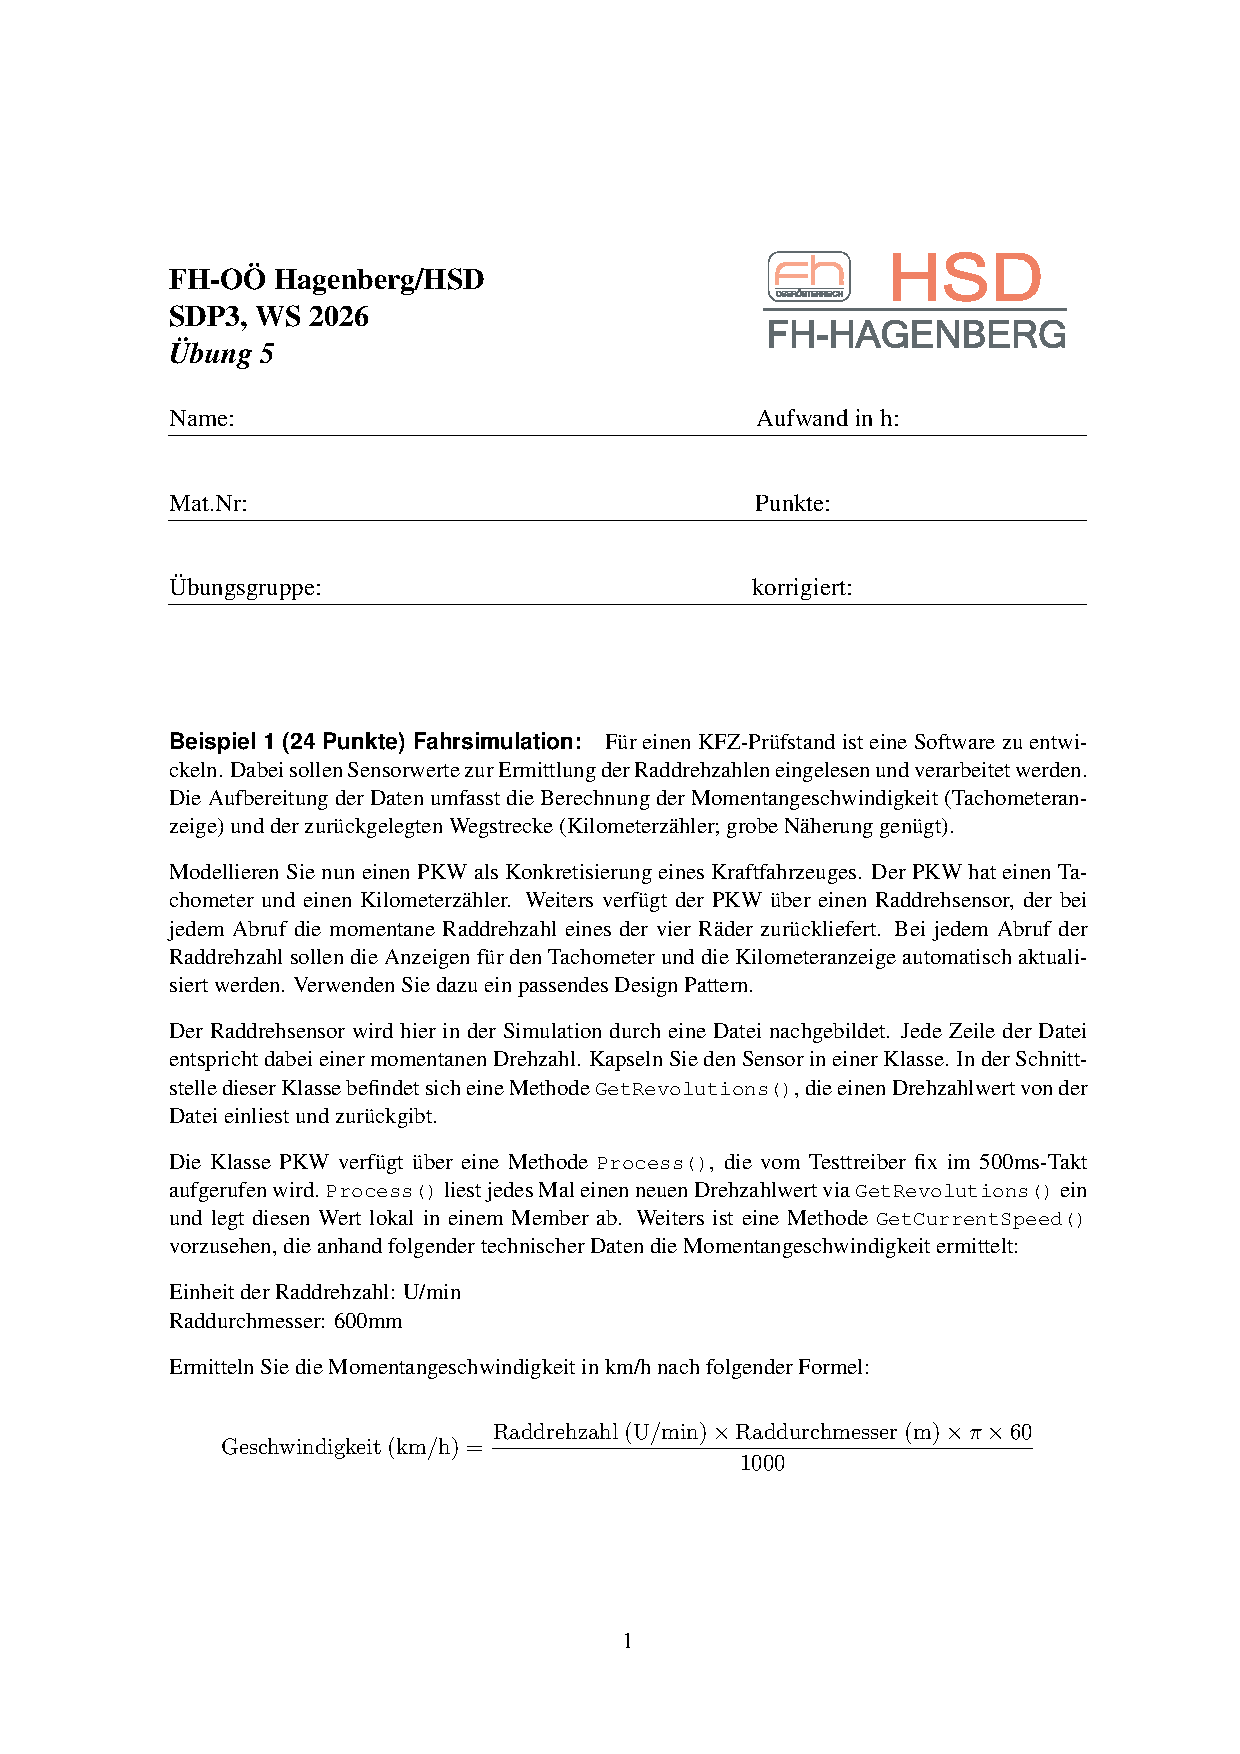
\includepdf[pages=-]{Angabe.pdf}
\newpage
\hgbtitle
\newpage


%%%%%%%%%%%%%%%%%%%%%%%%%%%%%%% Inhaltsverzeichnis %%%%%%%%%%%%%%%%%%%%%%%%

\tableofcontents
\newpage

%%%%%%%%%%%%%%%%%%%%%%%%%%%%%%% Ausarbeitung %%%%%%%%%%%%%%%%%%%%%%%%%%%%%%

\section{Organisatorisches}

\subsection{Team}
\begin{itemize}
	\item \docauthor, Matr.-Nr.: \docauthornumber, E-Mail: \docauthoremail	
	\item \doccoauthor, Matr.-Nr.: \doccoauthornumber, E-Mail: \doccoauthoremail
\end{itemize}

\subsection{Aufteilung der Verantwortlichkeitsbereiche}
\begin{itemize}
	\item \docauthor
	\begin{itemize}
		\item Klassendiagramm
		\item Anforderungsdefinition
		\item Implementierung und Unit-Test:
		\begin{itemize}
			\item IWheelSpeedSensor
			\item WheelSpeedSimulator
			\item IVehicleListener
			\item Display
			\item Speedometer
			\item KilometerCounter
		\end{itemize}
	\end{itemize}
	\item \doccoauthor
	\begin{itemize}
		\item Designentscheidungen
		\item Implementierung und Unit-Test:
		\begin{itemize}
			\item Object
			\item Vehicle
			\item MotorVehicle
			\item Car
			\item ISpeedProvider
		\end{itemize}
	\end{itemize}	
\end{itemize}

\subsection{Aufwand}

\begin{itemize}
	\item \docauthor: geschätzt 7 Ph / tatsächlich 6 Ph
	\item \doccoauthor: geschätzt 7 Ph / tatsächlich 6 Ph
\end{itemize}

\section{Anforderungsdefinition (Systemspezifikation)}
 
 Das Ziel ist es, eine Software zu entwickeln, mit der Daten von Fahrzeugen (in diesem Fall einem PKW) auf einem Fahrzeug-Prüfstand gespeichert werden können. Dabei wird über einen Raddrehsensor die Drehzahl von einem der Räder gemessen und basierend darauf die Momentangeschwindigkeit und die insgesamt am Prüfstand gefahrenen Kilometer ausgegeben.\\
 Die Ausgabe und Visualisierung der Daten soll von zwei fertigen Display-Programmen durchgeführt werden.
 Alle 500ms soll der Sensor überprüft, und die Daten aktualisiert werden. Ein PKW hat einen fixen Raddurchmesser von 600mm. 
 
\section{Systementwurf}

\subsection{Klassendiagramm}
\fig{Systemdoku/Images/Fahrsimulation.png}{1.2}{Klassendiagramm \docproject}

\subsection{Designentscheidungen}

\textbf{Object} wird wieder als Basisklasse aller Basisklassen verwendet, damit der virtuelle Destruktor überall vorhanden ist.\\

Die abstrakte Klasse \textbf{Vehicle} bildet das Subjekt im \textbf{Observer Pattern}. Sie verwaltet ein Vector von \textbf{IVehicleListener}n (Member \textit{mListeners}), die über die öffentliche Methode \textit{Register} hinzugefügt werden können. Über die protected Methode \textit{Notify} werden alle registrierten Listener über Zustandsänderungen informiert, indem deren \textit{Update}-Methode aufgerufen wird.\\

Die abstrakte Klasse \textbf{MotorVehicle} erbt von \textbf{Vehicle} und implementiert gleichzeitig das Interface \textbf{ISpeedProvider}. Sie kapselt die physikalischen Eigenschaften und den Zustand eines Kraftfahrzeugs, konkret den Reifendurchmesser (\textit{mTireDimension}) und die aktuellen Radumdrehungen (\textit{mRevs}). Um die Radumdrehungen auszulesen, hält sie eine Komposition zu einem \textbf{IWheelSpeedSensor} (\textit{mWheelSpeedSensor}), der beim Konstruieren übergeben wird. In der Methode \textit{Process} wird die aktuellem Daten vom WheelSpeedSensor eingelesen und gespeichert. Anschließend werden über \textit{Notify} die Listener über neue Werte benachrichtigt. Über \textit{GetCurrentSpeed} wird anhand der Umdrehungen und des Reifendurchmessers die aktuelle Geschwindigkeit des Fahrzeuges berechnet.\\

Die konkrete Klasse \textbf{Car} erbt von \textbf{MotorVehicle} und legt im Konstruktor einen fixen Reifendurchmesser fest, während der \textbf{IWheelSpeedSensor} an den Konstruktor von \textbf{MotorVehicle} weitergereicht wird.\\

Für die Erfassung der Radumdrehungen definiert das Interface \textbf{IWheelSpeedSensor} die Methode \textit{GetRevolutions}. Die konkrete Klasse \textbf{WheelSpeedSimulator} implementiert dieses Interface. Sie liest die Umdrehungswerte über einen Dateistream (\textit{mFile}) aus einer im Konstruktor übergebenen Datei aus.\\

Auf der Seite der Beobachter erben die konkreten Anzeigeklassen \textbf{KilometerCounter} und \textbf{Speedometer} sowohl von der abstrakten Klasse \textbf{Display} als auch vom Interface \textbf{IVehicleListener}. Beide halten jeweils eine Referenz auf einen \textbf{ISpeedProvider} (\textit{mProvider}), um bei einem Aufruf ihrer \textit{Update}-Methode die aktuelle Geschwindigkeit abzufragen. \textbf{Speedometer} gibt diesen Wert direkt an das Display weiter, während \textbf{KilometerCounter} zusätzlich die gefahrenen Kilometer in \textit{mKilometers} aufsummiert.\\

Die abstrakte Klasse \textbf{Display} kapselt die Darstellung über ein \textbf{WindowsDisplay}-Objekt (\textit{mDisplay}). \textbf{WindowsDisplay} ist selbst abstrakt, erbt von \textbf{Object} und übernimmt die Kommunikation über Windows-Pipes (\textit{mhPipe}) mittels der Methode \textit{SendValue}. Die konkreten Unterklassen \textbf{DigitalDisplay} und \textbf{AnalogDisplay} übergeben im Konstruktor lediglich den jeweiligen Pipe-Namen an den Konstruktor von \textbf{WindowsDisplay}, um die unterschiedliche Visualisierung zu realisieren.\\

Durch die vielen Interfaces ist das Design leicht erweiterbar. Man könnte einfach neue Klassen hinzufügen, beispielsweise \textbf{Moped}, \textbf{RealWheelSpeedSensor} oder \textbf{AvgSpeedDisplay}.\\

\section{Dokumentation der Komponenten (Klassen)}

Die HTML-Startdatei befindet sich im Verzeichnis \href{run:./../doxy/html/index.html}{./../doxy/html/index.html}

\section{Dateibeschreibung}

Die Struktur der Radumdrehungs-Datei muss folgendermaßen aussehen:
\testoutput{Systemdoku/EBNF}
In jeder Zeile der Datei steht genau eine Umdrehungszahl $\rightarrow$ also mit newline getrennt (nicht in EBNF).

\section{Testprotokollierung}
Die Unit- und Systemtests wurden wieder mit Google Test Suite durchgeführt. Vor dem Starten der Tests müssen die beiden Display Programme geöffnet und ggf. der Server neu gestartet werden. Die Funktionalität ist teilweise visuell zu überprüfen, da die Programme keine bessere Anbindungsmöglichkeit bieten.

\testoutput{Systemdoku/Tests}

\section{Quellcode}
\subsection{Object}
\h{Beispiel01/Object}

\subsection{ISpeedProvider}
\h{Beispiel01/ISpeedProvider}

\subsection{IWheelSpeedSensor}
\h{Beispiel01/IWheelSpeedSensor}

\subsection{WheelSpeedSimulator}
\cppmodule{Beispiel01/WheelSpeedSimulator}

\subsection{Vehicle}
\cppmodule{Beispiel01/Vehicle}

\subsection{MotorVehicle}
\cppmodule{Beispiel01/MotorVehicle}

\subsection{Car}
\cppmodule{Beispiel01/Car}

\subsection{IVehicleListener}
\h{Beispiel01/IVehicleListener}

\subsection{Display}
\h{Beispiel01/Display}

\subsection{KilometerCounter}
\cppmodule{Beispiel01/KilometerCounter}

\subsection{Speedometer}
\cppmodule{Beispiel01/Speedometer}

\subsection{Testtreiber}
\cpp{Beispiel01/Test}

\end{document}
%%%%%%%%%%%%%%%%%%%%%%%%%%%%%%%%%%%%%%%%%%%%%%%%%%%%%%%%%%%%%%%%%%%%%%%%%%%